\chapter{Related work}

\section{U-Net: Convolutional Networks for Biomedical
Image Segmentation} \label{unet}

    In this part, we introduce the architecture of the model that is the foundation of the work in this thesis, and hence in  more detailed. U-Net is a fully convolutional state-of-the-art\cite{rajak2021segmentation} semantic segmentation \gls{cnn} and was initially developed for biomedical image analysis by \citeauthor{unet_ronneberger2015}\cite{unet_ronneberger2015}. 
    
    \begin{figure}[H]
        \centering
        %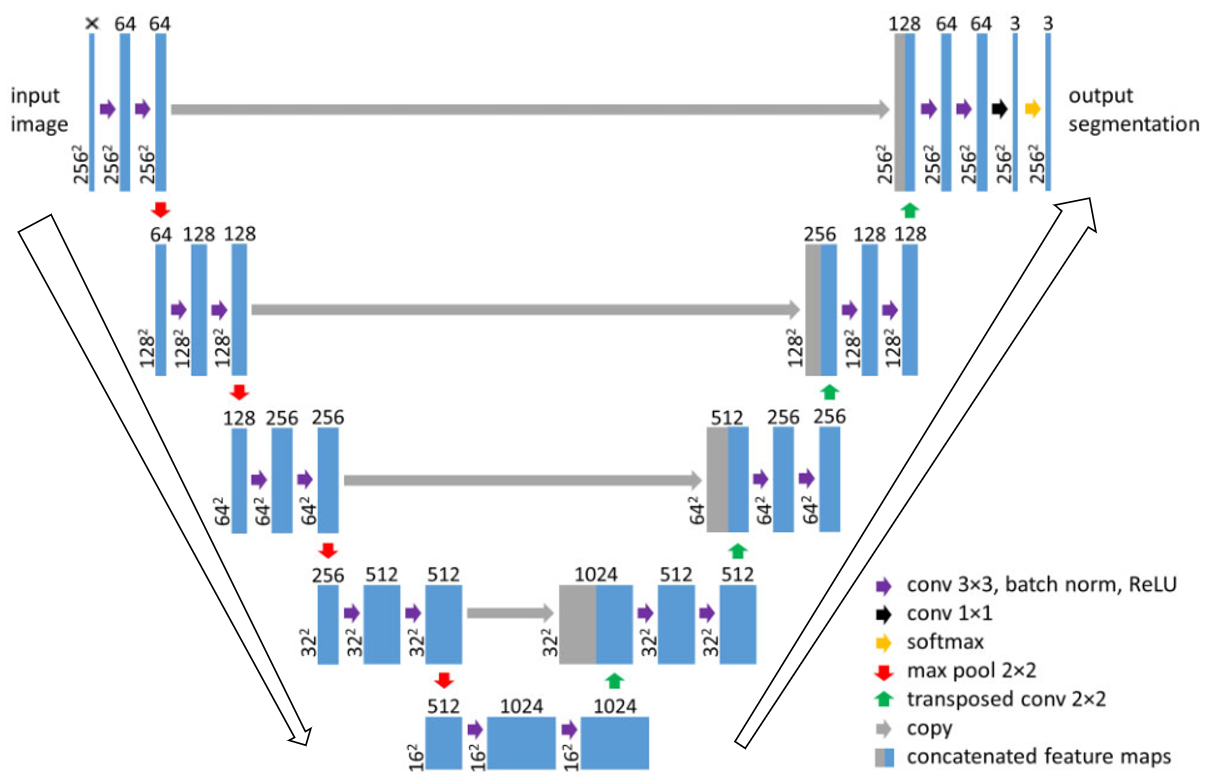
\includegraphics[scale=0.5]{figures/unet_arrows.png}
        \includesvg[inkscapelatex=false,width=1.0\textwidth,keepaspectratio]{figures/unet_original.svg}
        \caption[U-Net architecture]{U-Net architecture, the downwards facing arrow illustrates the contracting path and the one facing upwards is the expanding path. The color gets darker as the channels increase.}
      	\medskip 
        \label{unet_fig}
        \hspace*{15pt}\hbox{\scriptsize Credit: \citeauthor{unet_ronneberger2015}\cite{unet_ronneberger2015}}
    \end{figure}
    
    Unet utilized what \citeauthor{unet_ronneberger2015}\cite{unet_ronneberger2015} called a contracting path to identify what was in a picture, while an expanding path to localize where it was. These two branches were symmetrical, and together they formed a U-shape, giving the network its name. The contracting path can be looked at as five different stages of processing, from top to bottom, in figure \ref{unet_fig}. Each stage applied the same operations to its given input. For each stage, this consisted of two 3×3 valid convolutions with their individual ReLU activation functions. Initially, the feature channels would be increased to 64, and later doubled for each contracting stage. The convolutions were followed by a 2×2 max pooling operation with stride 2 to decrease the resolution of the output from the convolutional operations, and then send this feature map down to the next stage. At the bottom stage, the only change was the use of transpose convolutions instead of max pooling to now increase the resolution. At each subsequent stage going back up the expanding path, the number of feature channels were halved during the convolutional steps. The output of the previous stage would be concatenated with a crop from the output feature map of a stage from the contracting path with the same channel size, the cropping due to different resolutions. This step is crucial for the performance of the model, as it helps the network localize the abstract features in the expanding path to locations in the contracting. At the last stage, a 1×1 convolution was applied instead of increasing the resolution. The 1×1 convolution mapped the 64 feature channels to the 2 classes. The softmax was then calculated between these classes, giving each pixel a value between [0,1], summarized over all classes to 1. Hence, giving us a segmentation map of each class. In the field of biomedicine, data are scarce and so heavy use of data augmentation was applied, which made the U-Net able to train on very few samples.
    
    As of U-Net's development in \citeyear{unet_ronneberger2015}, it outperformed other networks in multiple biomedical challenges\cite{unet_ronneberger2015}. It's performance inspired new versions with enhanced performance that use the U-Net architecture as its backbone, as can be seen in NAS-Unet\cite{weng2019unet} from \citeyear{weng2019unet}, and Unet++\cite{zhou2018unet} from \citeyear{zhou2018unet}. U-Net has also been applied with success to other fields such as road extraction in satellite images by \citeauthor{zhang2018road}\cite{zhang2018road} in \citeyear{zhang2018road} and on acoustic classification by \citeauthor{brautaset2020acoustic}\cite{brautaset2020acoustic} in \citeyear{brautaset2020acoustic}, which is the next article to be described in this thesis.
    
    
\section{Acoustic classification in multifrequency echosounder data using deep convolutional neural networks} \label{unet_paper_acoustic}
    
    
    OBS! Må ha forklart U-net, accoustic klassifikasjon, F1 OBS, feature construction, statistical and machine learning methods!
    
    To help assess the size of legal fishing quotas, acoustic trawls surveys are initiated to gather data. Before the data is of use, an operator manually needs to interpret the data in a time-consuming process to assign the acoustic back scattering to the correct category, but in turn often introduces bias. Several methods have been implemented to reduce this bias and with a goal to automate the process, but they all have a common weakness where they need a predefined feature space.  In 2020 a group of researchers implemented a U-net deep learning model to the problem and as this is an \gls{cnn} it does not need to have pre-designed features but learn them from the data. Sandeel  ~\cite{brautaset2020acoustic}. 
    
    %In this thesis, this will be a semantic segmentation of the classes \textit{background}, \textit{other } and most importantly \textit{sandeel}.
    
    
    
    The \gls{crimac} used this model in their project (described in \ref{unet_paper_acoustic}) and had to do some small modifications to the network to fit their task. This modified U-Net is the one presented in this section, as this is the one used in the experiments. The core functionality of the network stays true to the original Unet, and the alterations done to the original will be explained later in this section.
    
    
    
    
    %Minor changes were made to adapt\citeauthor{unet_ronneberger2015}s original U-Net to the acoustic data used in \ref{unet_paper_acoustic}, as the input now had the form 4 x 256 x 256. The four channels being the frequencies used. The convolutions were set to \textit{same} instead of \textit{valid}, as were the original setting. This was done to make the size of the input and output match. Further, batch normalization was added to each convolution. 
    
    \subsection{Result}
        things
    \subsection{Problems}